\section*{Component design}
In the following sections we will describe and explain our component diagrams of the system, and how the different components interact throughout the system.
\subsection*{Toll lanes}
In \autoref{fig:ComponentDiagram_TollLane} we show the toll lane components. In the diagram four main components are shown, namely Express Check-in Toll Lane, Express Check-out Toll Lane, Normal Check-out Toll Lane and Normal Check-in Toll Lane. These components describe the software present in the different kind of toll lanes, and how they interface with their needed hardware components, such as Antenna and Ticket Reader, and then how these interfaces with different actors. Interfaces to the other parts of the system is split up and described in other diagrams to keep the complexity down in this diagram.
\begin{figure}[H]
\centering
\includegraphics[width=0.7\linewidth]{img/component_diagram/ComponentDiagram_TollLane.png}
\caption{Component diagram for toll lanes}
\label{fig:ComponentDiagram_TollLane}
\end{figure}

\subsection*{Toll station}
In \autoref{fig:ComponentDiagram_TollLaneToStationAndEnterprise} the component diagram for the toll station is shown. The toll station component contains the toll lanes and the toll station server component. When the lanes have to communicate with the enterprise server it is done through the toll station server component. The main thing to communicate out of the toll station component is toll tag data, and data for the reports the enterprise manager can generate.
\begin{figure}[H]
\centering
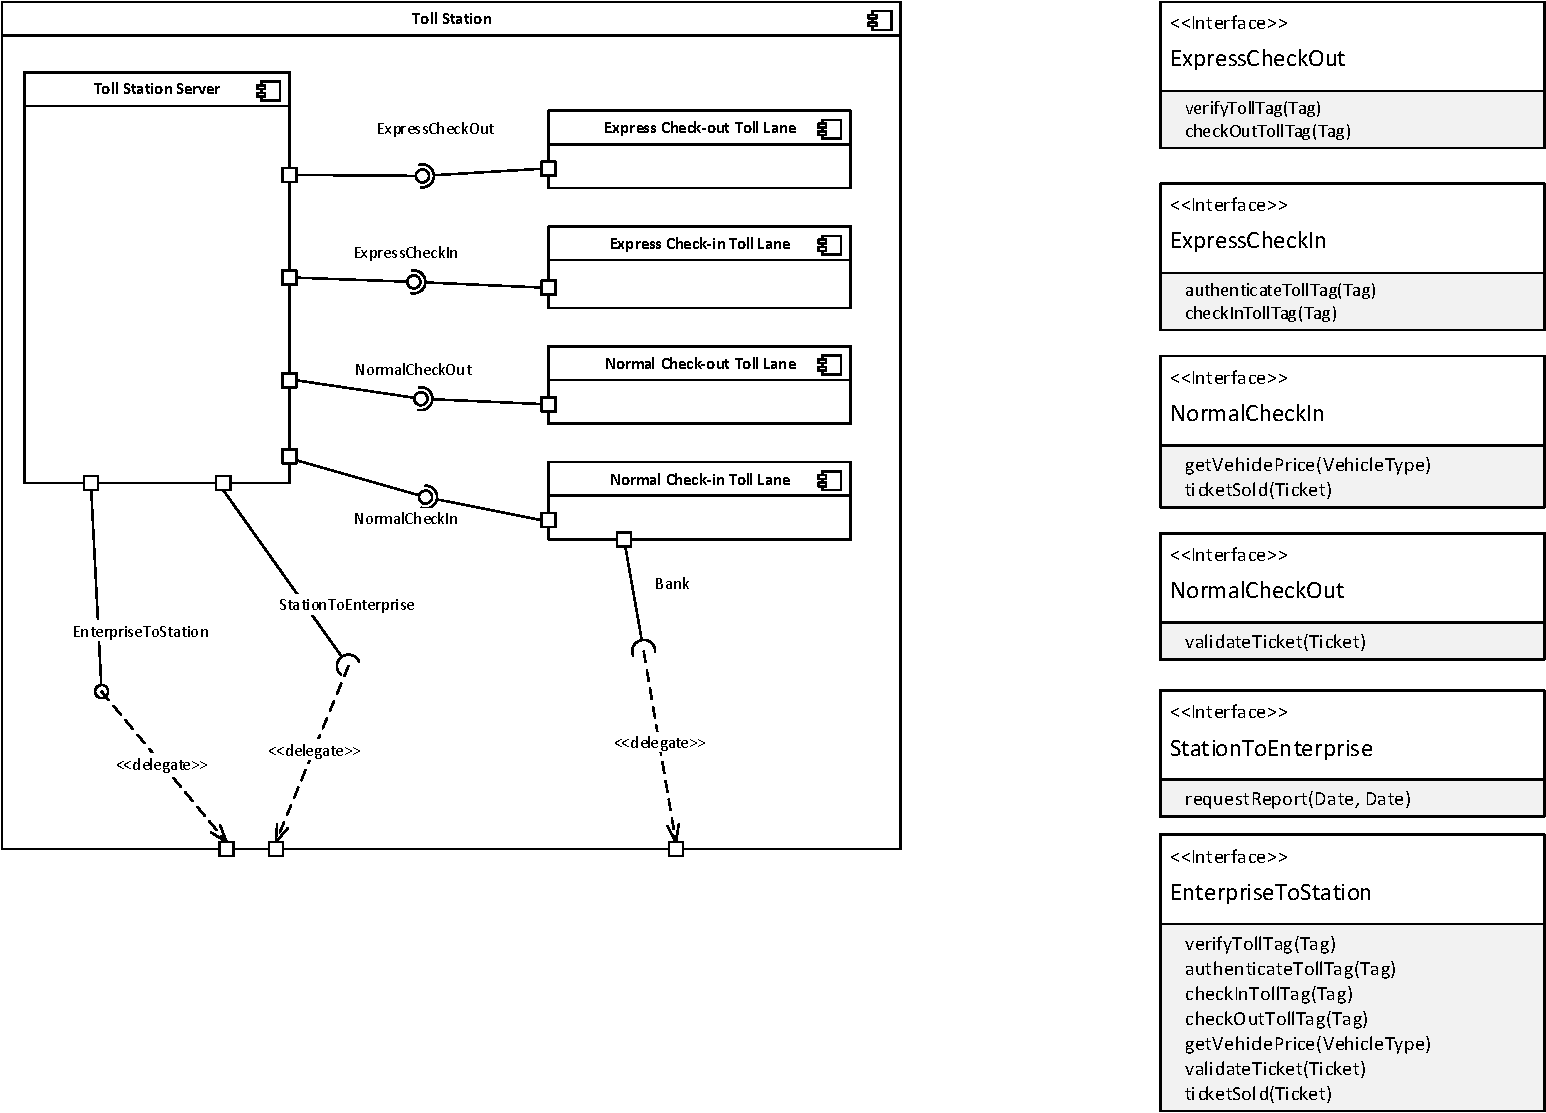
\includegraphics[width=0.7\linewidth]{img/component_diagram/ComponentDiagram_TollLaneToStationAndEnterprise.png}
\caption{Component diagram for toll station}
\label{fig:ComponentDiagram_TollLaneToStationAndEnterprise}
\end{figure}

\subsection*{Enterprise server}
Finally, in \autoref{fig:ComponentDiagram_Enterprise} we show the simple component diagram for the enterprise server, along with the most macroscopic view of our system. 
\begin{figure}[H]
\centering
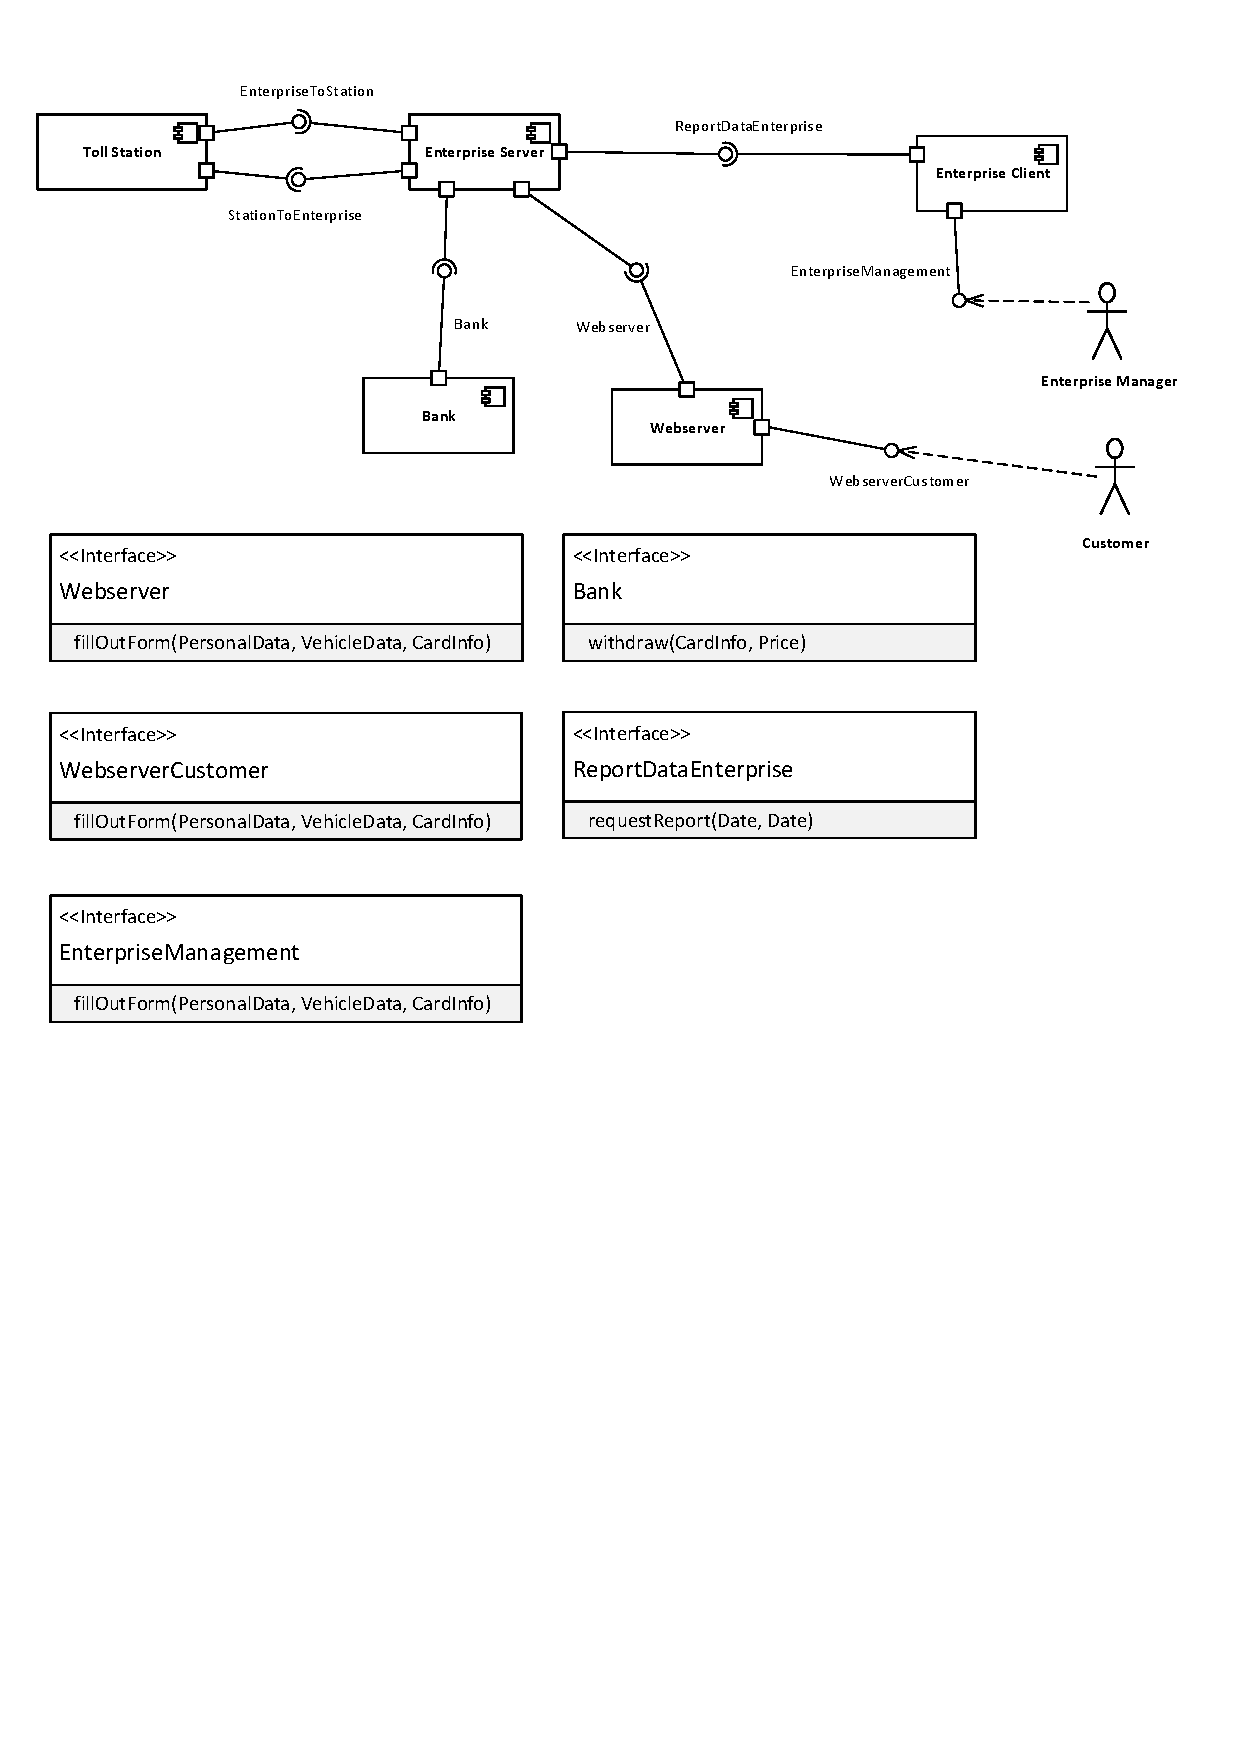
\includegraphics[width=0.7\linewidth]{img/component_diagram/ComponentDiagram_Enterprise.png}
\caption{Component diagram for enterprise}
\label{fig:ComponentDiagram_Enterprise}
\end{figure}
